\documentclass{beamer}
\usetheme[]{Copenhagen}

\usepackage[french]{babel}
\usepackage{caption}
\captionsetup[figure]{labelformat=empty}% redefines the caption setup of the figures environment in the beamer class.

\addtobeamertemplate{navigation symbols}{}{%
	\usebeamerfont{footline}%
	\usebeamercolor[fg]{footline}%
	\hspace{1em}%
	\insertframenumber/\inserttotalframenumber
}

\title{Simulateur du Jeu de la vie}
\author{DAVID Matthias, LE BRIS Ilan, MARCHERON Bastien, PARCHEMINER Nolann}
\institute{Université de Caen Normandie}
\date{\today}
\logo{
\includegraphics[height=1cm]{image/logo_unicaen.png}}

\begin{document}
	\frame{\titlepage}
	
	\begin{frame}{John Horton Conway}
		\begin{columns}
			% Column 1
			\begin{column}{0.5\textwidth}
				Mathématicien (1937-2020), inventeur du Jeu de la vie en 1970.
			\end{column}
			% Column 2    
			\begin{column}{0.5\textwidth}
				\begin{figure}
					\centering
					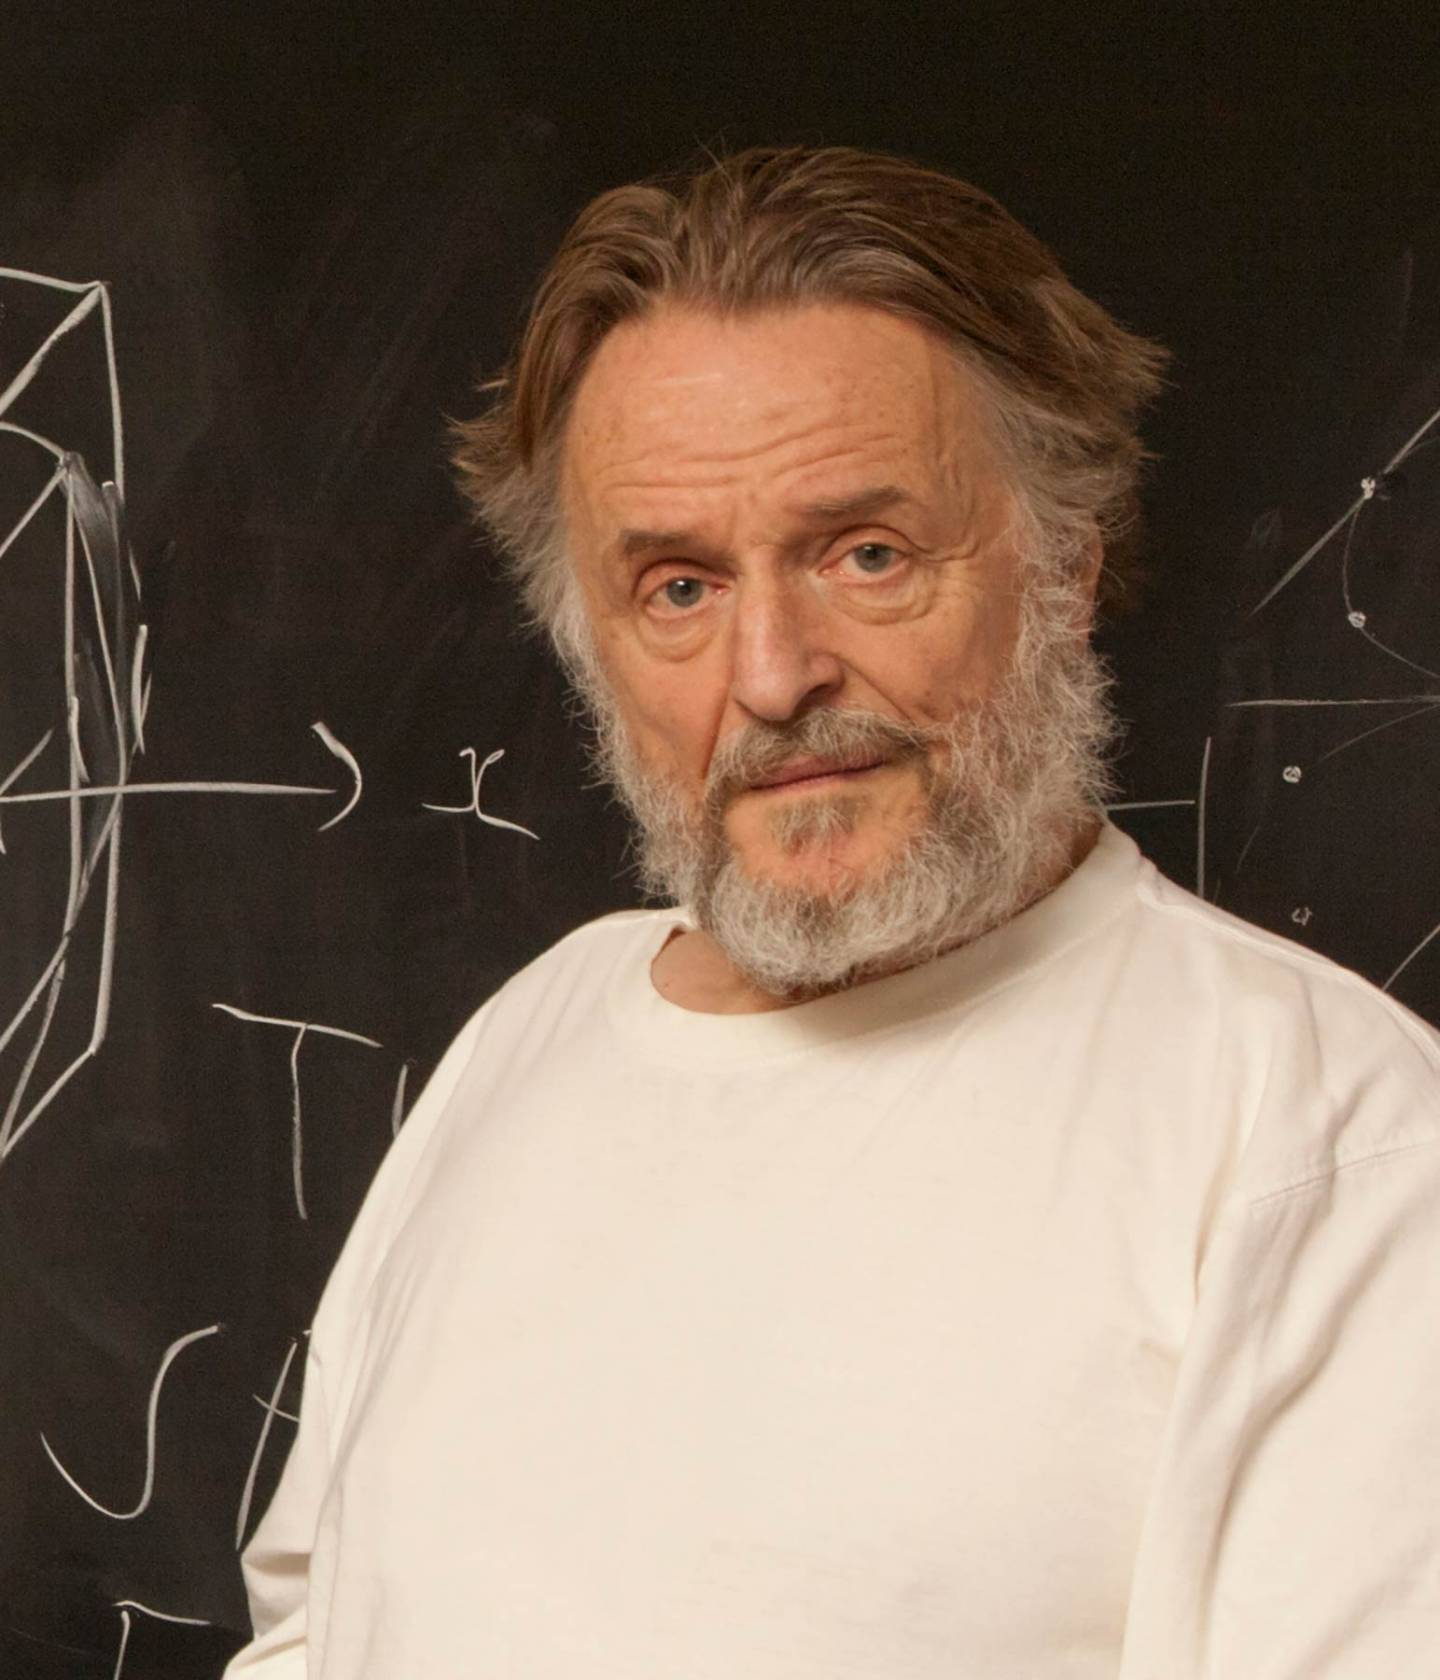
\includegraphics[width=0.7\textwidth]{image/Conway.jpg}
				\end{figure}
			\end{column}
		\end{columns}
	\end{frame}

	\begin{frame}{Fonctionnalités implémentées}{Obligatoire}
		\begin{itemize}
			\item Java
			\item Système de gestion de version
			\item Scripts de compilation
			\item Implémentation d'automates cellulaires
			\item Implémenter l'algorithme HashLife
			\item Fournir une interface configurable
			\item Tests unitaires
		\end{itemize}
	\end{frame}

	\begin{frame}{Fonctionnalités implémentées}{Optionnelles}
		\begin{itemize}
			\item Fichiers de configurations
			\item Zoom/dé-zoom sur la grille
			\item Translation vertical et horizontal
			\item Interface responsive
			\item Sauvegarde de l'état en image		
		\end{itemize}
	\end{frame}

	\begin{frame}{Analyse de la charge de travail}
	    4 points essentiels : 	
		\begin{itemize}
			\item \textbf{Core : }C\oe ur de l'application
			\item \textbf{GUI : }Éléments de l'interface graphique
			\item\textbf{Utils : }Gestion des fichiers de sauvegarde
			\item \textbf{Tests : }Création de tests unitaires
		\end{itemize}
	\end{frame}

	\begin{frame}{ANT}
		\begin{itemize}
			\item Initialisation
			\item Compilation
			\item Lancement des tests
			\item Exécution 
			\item Génération de la documentation
			\item Nettoyage des fichiers de compilation
			\item Construction du projet final (distribution)
		\end{itemize}
	\end{frame}

	\begin{frame}{Structure de l'application}
		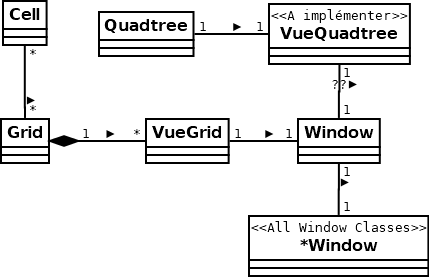
\includegraphics[width=0.8\textwidth]{image/diagramme.png}
	\end{frame}

	\begin{frame}{Utilisation des Threads}
		Permet de gérer en parallèle le calcul de génération des cellules et les éléments de l'interface graphique.
	\end{frame}

	\begin{frame}{Implémentation de HashLife}
		HashLife est un algorithme de génération de cellules puissant se basant sur les Quadtree.\\
		\vspace{0.2in}
		Cet algorithme a été implémenté dans notre projet, cependant il manque une classe "VueQuadtree" qui permettrai d'afficher un Quadtree sur notre interface graphique
	\end{frame}

	\begin{frame}{Les fichiers de configuration}{Les profiles}
		\begin{figure}
			\caption{Extension \emph{.gol.profile}}	
			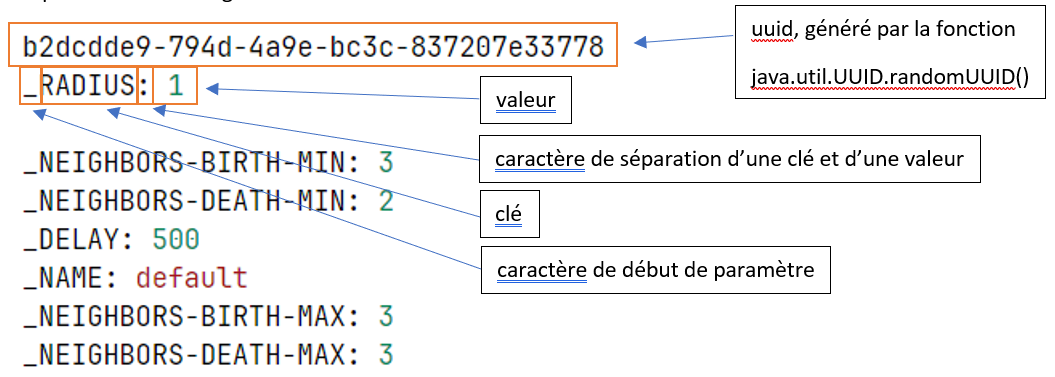
\includegraphics[width=0.8\textwidth]{image/profiles.png}
		\end{figure}
	\end{frame}

	\begin{frame}{Les fichiers de configuration}{Les presets}
		\begin{figure}
			\caption{Extension \emph{.gol.preset}}	
			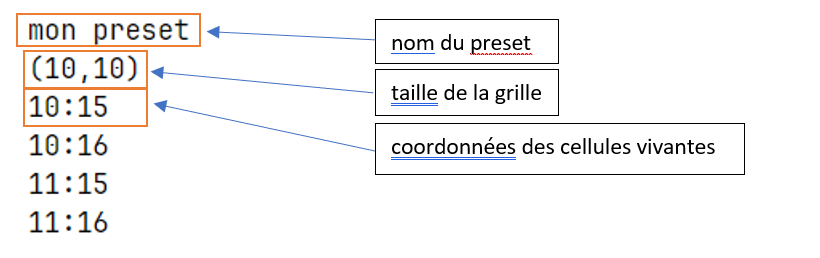
\includegraphics[width=0.8\textwidth]{image/presets.png}
		\end{figure}
	\end{frame}

	\begin{frame}{Test unitaires}
		L'avantage de faire des tests est d'avoir une vue plus globale du projet, ainsi que de déceler certains problèmes et de les corriger. 
	\end{frame}

	\begin{frame}{Améliorations possibles}
		Pour ce projet : 
		\begin{itemize}
			\item Résoudre quelque bugs sur l'interface graphique
			\item Implémenter une Vue sur les Quadtree
		\end{itemize}
		\vspace{0.4in}
		Pour des projets futurs : 
		\begin{itemize}
			\item Une meilleure préparation en amont
			\item Perfectionner notre utilisation de Git 
		\end{itemize}
	\end{frame}
	
	\begin{frame}{Conclusion}
		Le projet a bien évolué comparé aux ébauches des premières séances.
		\begin{center}
			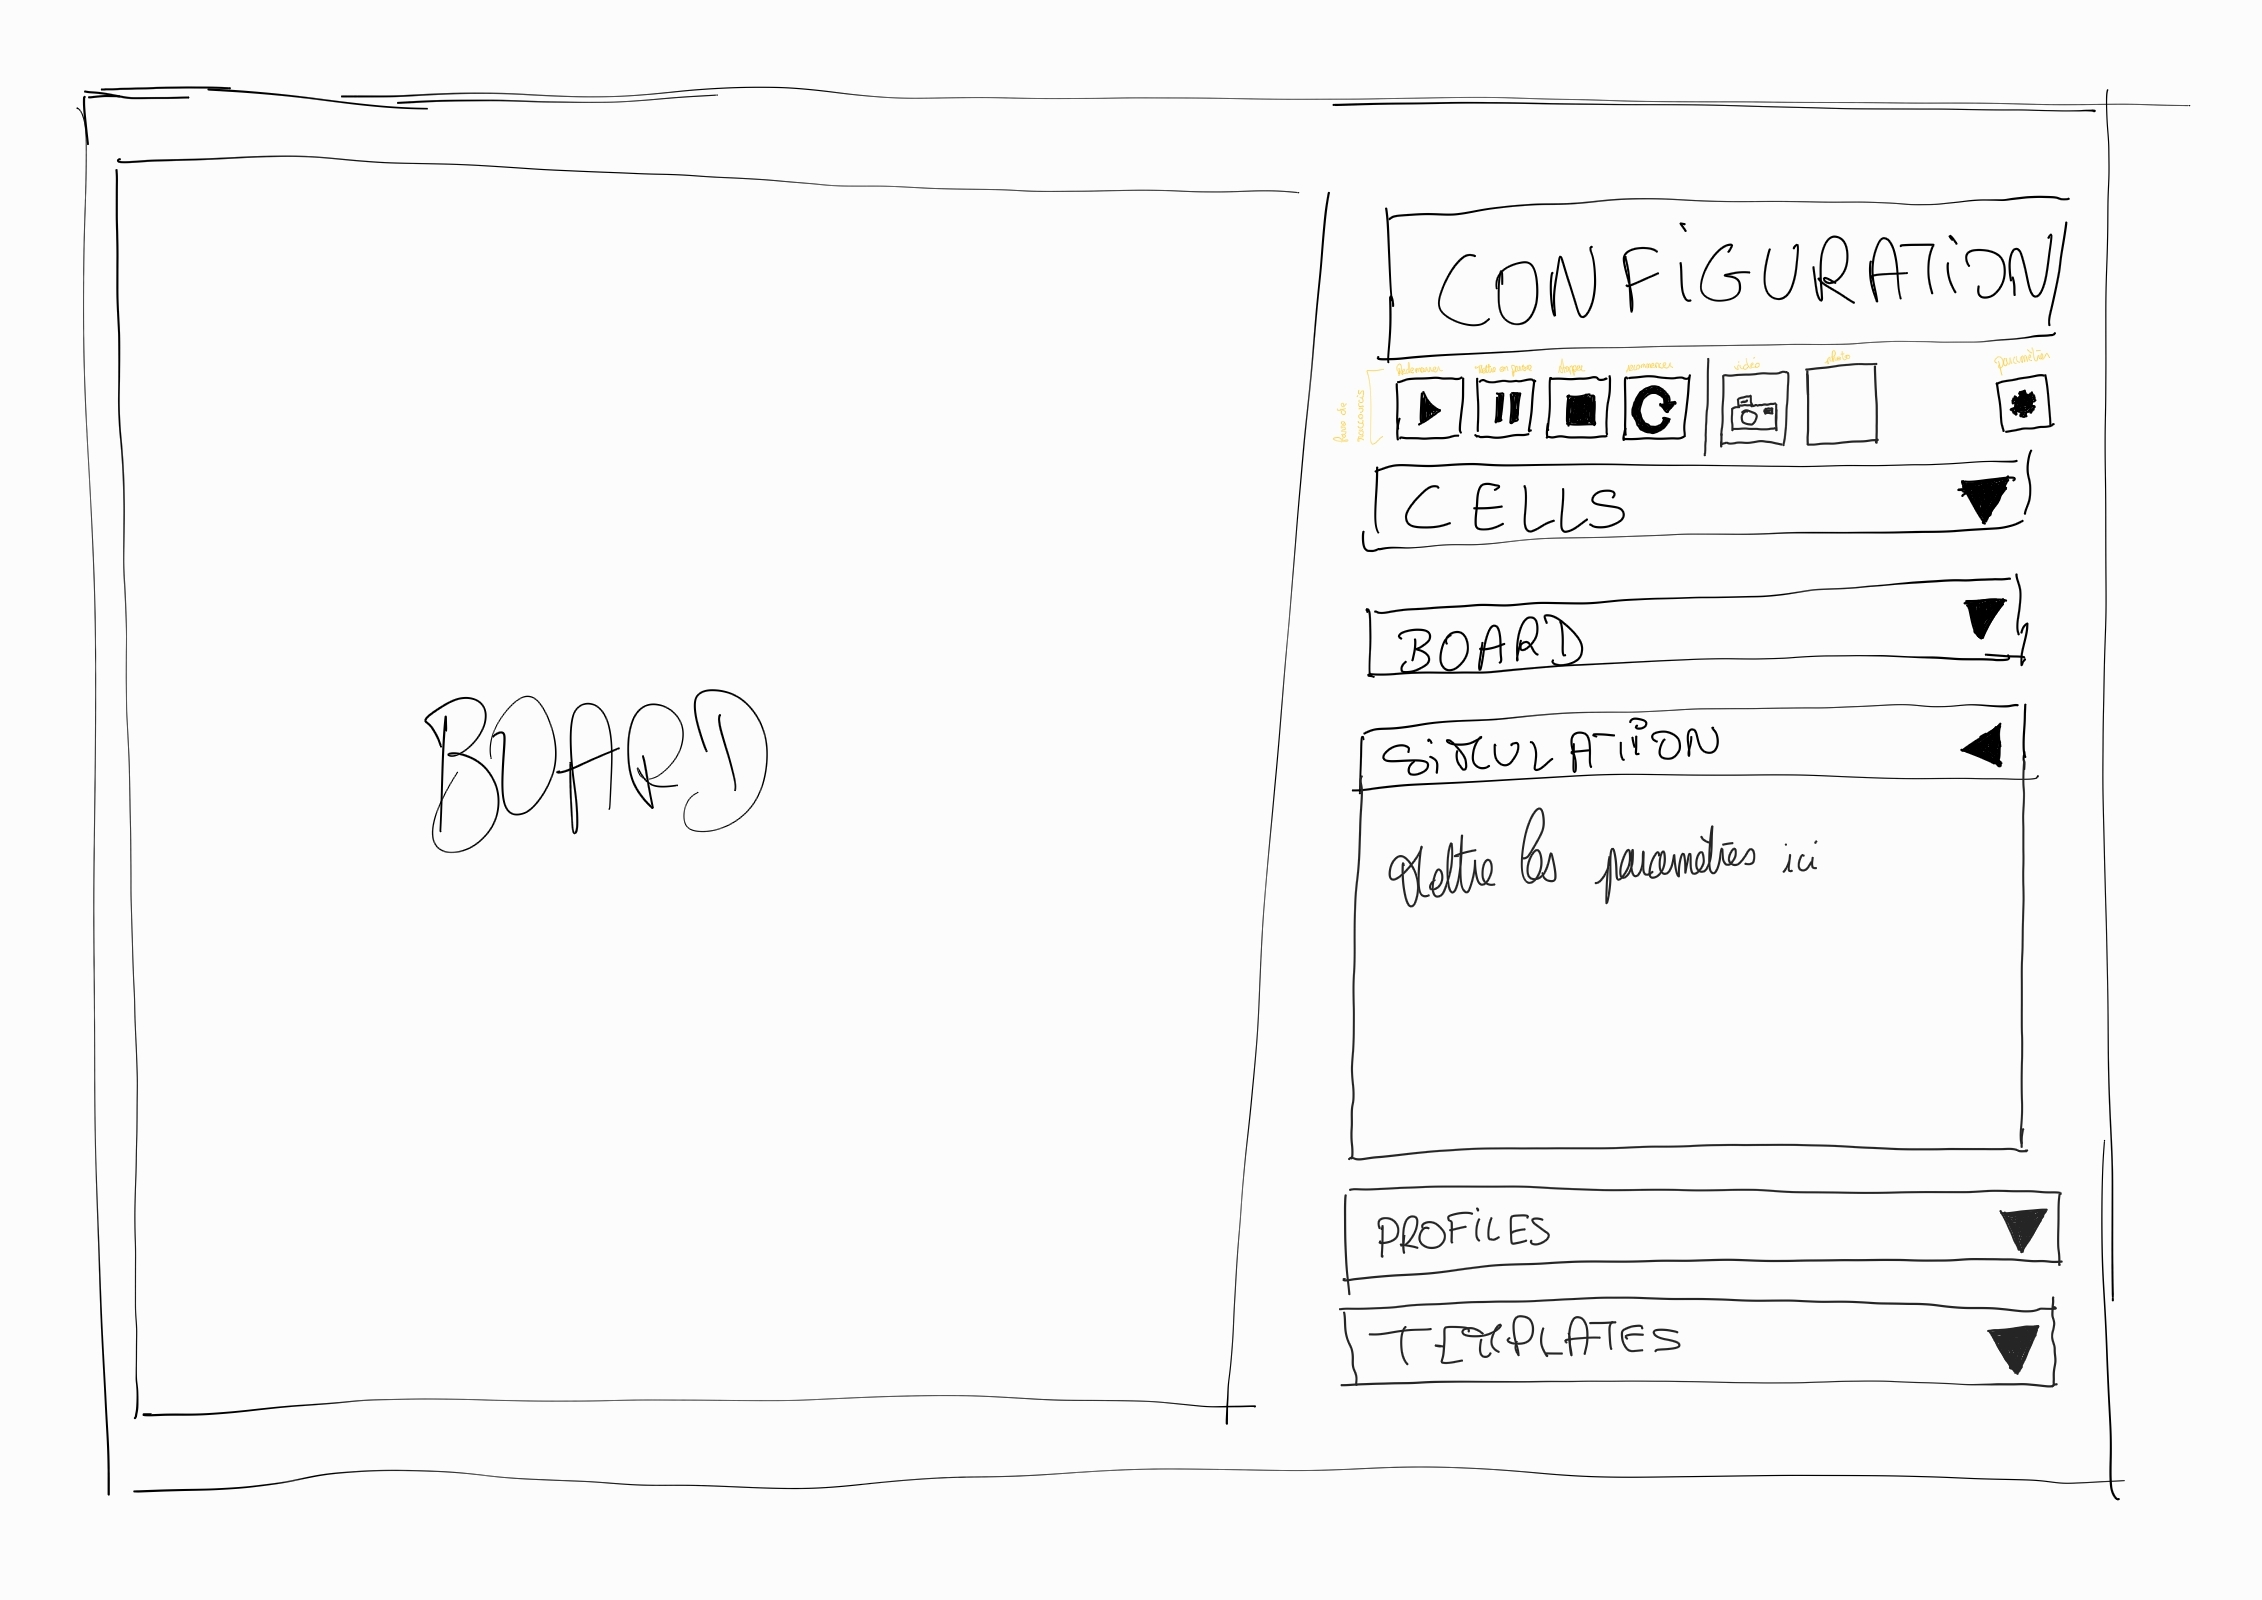
\includegraphics[height=0.4\textheight]{image/ebauche.jpg}	
		\end{center}
		Il nous a permis d'apprendre à utiliser divers outils (Git, ant, dia), très utiles pour nos prochains projets.
		
	\end{frame}
	
\end{document}